\documentclass[
  bibliography=totoc,     % Literatur im Inhaltsverzeichnis
  captions=tableheading,  % Tabellenüberschriften
  titlepage=firstiscover, % Titelseite ist Deckblatt
]{scrartcl}

% Paket float verbessern
\usepackage{scrhack}

% Warnung, falls nochmal kompiliert werden muss
\usepackage[aux]{rerunfilecheck}

% unverzichtbare Mathe-Befehle
\usepackage{amsmath}
% viele Mathe-Symbole
\usepackage{amssymb}
% Erweiterungen für amsmath
\usepackage{mathtools}

% Fonteinstellungen
\usepackage{fontspec}
% Latin Modern Fonts werden automatisch geladen
% Alternativ zum Beispiel:
%\setromanfont{Libertinus Serif}
%\setsansfont{Libertinus Sans}
%\setmonofont{Libertinus Mono}

% Wenn man andere Schriftarten gesetzt hat,
% sollte man das Seiten-Layout neu berechnen lassen
\recalctypearea{}

% deutsche Spracheinstellungen
\usepackage[ngerman]{babel}


\usepackage[
  math-style=ISO,    % ┐
  bold-style=ISO,    % │
  sans-style=italic, % │ ISO-Standard folgen
  nabla=upright,     % │
  partial=upright,   % ┘
  warnings-off={           % ┐
    mathtools-colon,       % │ unnötige Warnungen ausschalten
    mathtools-overbracket, % │
  },                       % ┘
]{unicode-math}

% traditionelle Fonts für Mathematik
\setmathfont{Latin Modern Math}
% Alternativ zum Beispiel:
%\setmathfont{Libertinus Math}

\setmathfont{XITS Math}[range={scr, bfscr}]
\setmathfont{XITS Math}[range={cal, bfcal}, StylisticSet=1]

% Zahlen und Einheiten
\usepackage[
  locale=DE,                   % deutsche Einstellungen
  separate-uncertainty=true,   % immer Unsicherheit mit \pm
  per-mode=symbol-or-fraction, % / in inline math, fraction in display math
]{siunitx}
\sisetup{range-phrase=--}       %bei Range --
% chemische Formeln
\usepackage[
  version=4,
  math-greek=default, % ┐ mit unicode-math zusammenarbeiten
  text-greek=default, % ┘
]{mhchem}

% richtige Anführungszeichen
\usepackage[autostyle]{csquotes}

% schöne Brüche im Text
\usepackage{xfrac}

% Standardplatzierung für Floats einstellen
\usepackage{float}
\floatplacement{figure}{htbp}
\floatplacement{table}{htbp}

% Floats innerhalb einer Section halten
\usepackage[
  section, % Floats innerhalb der Section halten
  below,   % unterhalb der Section aber auf der selben Seite ist ok
]{placeins}

% Seite drehen für breite Tabellen: landscape Umgebung
\usepackage{pdflscape}

% Captions schöner machen.
\usepackage[
  labelfont=bf,        % Tabelle x: Abbildung y: ist jetzt fett
  font=small,          % Schrift etwas kleiner als Dokument
  width=0.9\textwidth, % maximale Breite einer Caption schmaler
]{caption}
% subfigure, subtable, subref
\usepackage{subcaption}

% Grafiken können eingebunden werden
\usepackage{graphicx}

% schöne Tabellen
\usepackage{booktabs}

% Verbesserungen am Schriftbild
\usepackage{microtype}

% Literaturverzeichnis
\usepackage[
  backend=biber,
  style=alphabetic
]{biblatex}
% Quellendatenbank
\addbibresource{lit.bib}
\addbibresource{programme.bib}

% Hyperlinks im Dokument
\usepackage[
  german,
  unicode,        % Unicode in PDF-Attributen erlauben
  pdfusetitle,    % Titel, Autoren und Datum als PDF-Attribute
  pdfcreator={},  % ┐ PDF-Attribute säubern
  pdfproducer={}, % ┘
]{hyperref}
% erweiterte Bookmarks im PDF
\usepackage{bookmark}

% Trennung von Wörtern mit Strichen
\usepackage[shortcuts]{extdash}

\author{%
  Theodor Zies\\%
  \href{mailto:theodor.zies@tu-dortmund.de}{theodor.zies@tu-dortmund.de}%
  \and%
  Tom Troska\\%
  \href{mailto:tom.troska@tu-dortmund.de}{tom.troska@tu-dortmund.de}%
}
\publishers{TU Dortmund – Fakultät Physik}


\subject{V107}
\title{Das Kugelfall-Viskosimeter nach Höppler}
\date{%
  Durchführung: 23.11.2021
  \hspace{3em}
  Abgabe: 30.11.2021
}

\begin{document}

\maketitle
\thispagestyle{empty}
\tableofcontents
\newpage

\section{Zielsetzung}
\label{sec:Zielsetzung}
In diesem Versuch werden zwei gekoppelte Pendel untersucht. Ziel ist es, die Schwingungs- und Schwebungsdauern~$T$ und~$T_{\symup{S}}$, sowie die
Kopplungskonstante $\kappa$ zu bestimmen. Dafür werden gleichsinnige, gegensinnige und gekoppelte Schwingungen betrachtet.

\section{Theorie}
\label{sec:Theorie}
Wird ein Fadelpendel der Länge $l$ in dem Gravitationsfeld der Erde um einen kleinen Winkel $\varphi$ ausgelenkt, so ist die rücktreibende Kraft
proportional zur Auslenkung $x$ aus der Ruhelage. Hierbei handelt es sich somit um eine harmonische Schwingung die mit der Diffenentialgleichung für
den harmonischen Oszillator beschrieben werden kann. Die Kreisfrequenz $\omega$ und die Schwingungsdauer $T$ lauten dann
\begin{align}
    \omega &= \sqrt{\frac{g}{l}} \label{eq:Kreisfrequenz} \\
    T &= 2\symup{\pi}\sqrt{\frac{l}{g}}. \label{eq:Schwingungsdauer}
\end{align}

\section{Durchführung}
\label{sec:Durchführung}

\subsection{Aufgabe A}

Für die erste Aufgabe wird die Schaltung in \autoref{fig:Schaltbild A} verwendet.
Dabei wird wie in der Theorie bereits erläutert eine Rechteckspannung angelegt.

\begin{figure}
    \centering
    \includegraphics[height=10cm]{content/Durchführung - a.pdf}
    \caption{Schaltbild für Messung A \cite{v353}}
    \label{fig:Schaltbild A}
\end{figure}


Es wird der Verlauf der Kondensatorspannung $U_{C}(t)$ in Abhängigkeit der Zeit $t$ beobachtet.
Die Freqquenz der angelegten Rechteckspannung und die Ablenkgeschwindigkeit des Kathodenstrahls werden hierbei so eingestellt,
dass sich eine Änderung um den Faktor 5 bis 10 von $U_{C}(t)$ auf dem Oszilloskop ablesen lässt.
Anschließend wird das Bild des Oszilloskops fotografiert und in der Auswertung analysiert.

\subsection{Aufgabe B}

Nun wird das Schaltbild entsprechend  \autoref{fig:Schaltbild B} verändert und eine Wechselspannung angelegt.

\begin{figure} [H]
    \centering
    \includegraphics[height=10cm]{content/Durchführung - b.pdf}
    \caption{Schaltbild für Messung B \cite{v353}}
    \label{fig:Schaltbild B}
\end{figure}

Dabei ist die Frequenz variabel einstellbar, wobei die Amplitude der Wechselspannung identisch bleibt.
Es wird nun die Amplitude $A$ der Kondensatorspannung in Abhängigkeit der Frequenz $\omega"$ gemessen,
dabei wird $\omega"$ von 50Hz bis 100.000Hz, also über mehrere Zehnerpotenzen hinweg, variert.
Die Messwerte werden in einer Tabelle erfasst und anschließend ausgewertet.

\subsection{Aufgabe C}

Für diese Aufgabe wird die Schaltung aus Aufgabe B leicht verändert, sodass der Verlauf der Wechselspannung  $U_{G}(t)$
und der Kondensatorspannung $U_{C}(t)$ mit einem 2-Kanal Oszilloskop betrachtet werden können.
Das neue Schaltbild ist in \autoref{fig:Schaltbild C+D} zu sehen.

\begin{figure} [H]
    \centering
    \includegraphics[height=10cm]{content/Durchführung - c+d.pdf}
    \caption{Schaltbild für Messung C und D \cite{v353}}
    \label{fig:Schaltbild C+D}
\end{figure}

Gemessen werden nun die Periodendauer $b$ und der Abstand $a$ der Nulldurchgänge, aus denen in der Auswertung
der Phasenversatz ermittelt wird. In \autoref{fig:Phase messen} ist die geometrische Bedeutung von $b$ und $a$ skizziert.
Die Ergebnisse werden wie in Aufgabe B tabellarisch erfasst und ausgewertet.

\begin{figure} [H]
    \centering
    \includegraphics[height=10cm]{content/Durchführung - Phase_messen.pdf}
    \caption{Skizze zur Ermittlung des Phasenversatzes \cite{v353}}
    \label{fig:Phase messen}
\end{figure}

\subsection{Aufgabe D}

Zuletzt wird die Wirkung des RC-Kreises als Integrationsglied überprüft, dafür kann die Schaltung aus
Aufgabe C beibehalten werden. Es wird wie in der Theorie erklärt eine Wechselspannung mit
geigneter Frequenz $\omega >> 1/RC$ eingestellt.
Dabei werden 3 verschiedene Formen der Wechselspannung gewählt: Eine Rechteck-, Sinus und Dreieicksspannung.
Auf dem 2-Kanal Oszilloskop ist jeweils die Form der Kondensatorspannung $U_{C}(t)$ und die Form der gewählten
Wechselspannung $U_{G}(t)$ zu sehen.
Die 3 Bilder werden fotografiert und in der Auswertung analysiert.
\section{Auswertung}
\label{sec:Auswertung}
\subsection{Messung der Zeitkonstanten $RC$ über die Entladekurve}
Die Entladekurve des $RC$-Kreises wird mit einem Oszilloskop sichtbar gemacht, wie 
in \autoref{fig:aufgabe a - rechteckspannung} zu sehen ist. Die verwendete Frequenz beträgt $f=5\symup{kHz}$.
Im Folgenden werden Wertepaare \{$f [\symup{Hz}], U [\symup{V}]$\} mithilfe von eingezeichneten Hilfslinien abgelesen
(\autoref{fig:aufgabe a - gitter und hilfslinien}) und tabellarisch aufgeführt (\autoref{tab:aufgabe a}). Es ist zu beachten,
dass die Schrittweite von $t$ nicht gleichmäßig gewählt wird, da sich die Werte mit der gewählten Schrittweite mit
geringerem Fehler ablesen lassen.

\begin{figure}
  \centering
  \includegraphics[height=10cm]{content/Aufgabe a - Rechteckspannung.pdf}
  \caption{Entladekurve des Kondensators mit Vorwiderstand}
  \label{fig:aufgabe a - rechteckspannung}
\end{figure}

\begin{figure}
  \begin{subfigure}{0.48\textwidth}
    \centering
    \includegraphics[height=5cm]{content/Aufgabe a - Gitter.pdf}
    \caption{Entladekurve mit Koordinatensystem}
    \label{fig:aufgabe a - gitter}
  \end{subfigure}
  \hfill
  \begin{subfigure}{0.48\textwidth}
    \centering
    \includegraphics[height=5cm]{content/Aufgabe a - Hilfslinien.pdf}
    \caption{Entladekurve mit Hilfslinien}
    \label{fig:aufgabe a - hilfslinien}
  \end{subfigure}
  \caption{Entladekurve mit eingezeichnetem Koordinatensystem und Hilfslinien. Die %
    Skalierung wurde vorher durch Messung der Spannung der Rechteckspannung ermittelt.}
  \label{fig:aufgabe a - gitter und hilfslinien}
\end{figure}

\begin{table}
  \centering
  \caption{Darstellung der Messwertpaare, welche aus \autoref{fig:aufgabe a - gitter und hilfslinien} abgelesen wurden.}
  \label{tab:aufgabe a}
  \begin{tabular}{S[table-format=2.0] S[table-format=1.1]}
    \toprule
    {$s$ [$\symup{\mu s}$]} & {$U$ [V]} \\
    \midrule
    0 &  5,0 \\
    6	&  4,2 \\
    10 & 3,8 \\
    16 & 3,3 \\
    20 & 3,0 \\
    26 & 2,6 \\
    30 & 2,3 \\
    36 & 2,0 \\
    40 & 1,8 \\
    46 & 1,6 \\
    50 & 1,4 \\
    56 & 1,2 \\
    60 & 1,1 \\
    \bottomrule
  \end{tabular}
\end{table}

\begin{figure}
  \centering
  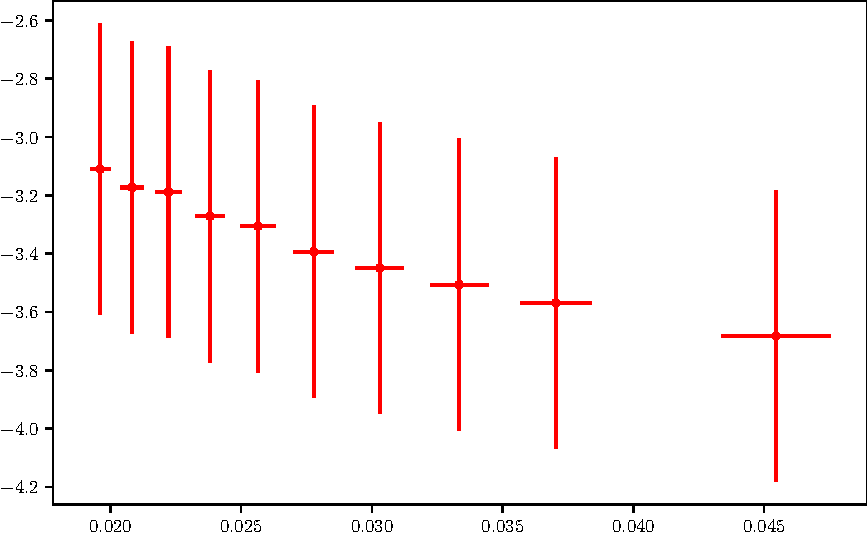
\includegraphics{build/plot_a.pdf}
  \caption{Halblogarithmischer Plot der Wertepaare aus \autoref{tab:aufgabe a} %
  mit Ausgleichsgerade.}
  \label{fig:plot_a}
\end{figure}

Mithilfe der Python-Erweiterungen "numpy" \cite{numpy} und "matplotlib" \cite{matplotlib} werden die Wertepaare der 
\autoref{tab:aufgabe a} halblogarithmisch geplottet und es wird eine Ausgleichsgerade eingezeichnet. Die Parameter der
Ausgleichsgerade vom Typ $ln(U) = m \cdot t + b$ werden zu $m=−0.025050069256648443$ und $b=1.5957959771629942$ bestimmt.
Die Formel des Entladevorgangs eines Kondensators
\begin{equation}
  U_{C} = U_{0}e^{-\frac{1}{RC}\cdot t}
\end{equation}
wird umgestellt zu
\begin{equation}
  ln(U) = ln(U_{0})-\frac{1}{RC}\cdot t
\end{equation}
und entspricht somit der Form der Ausgleichsgerade. Die Zeitkonstante $RC$ ist folglich 
$RC = \frac{1}{m} = 39.920049312222716 \symup{\mu s}$



\subsection{Bestimmung der Zeitkonstante $RC$ über die Frequenabhängigkeit der Amplitude}
Die Spannung am Kondensator $A$ wird ebenso wie die Spannung der Sinusspannungsquelle $U_{0}$ bei variabler
Frequenz $f$ gemessen und tabellarisch in \autoref{tab:aufgabe c} dargestellt. Da sich bei der Messung $U_{0}$
als frequenzunabhängig und zu $U_{0} = 5,2$V bestimmen lässt, ist dieser Wert aus Gründen der
Übersichtlichkeit nicht in der Tabelle aufgeführt. Das Teilungsverhältnis aus $\frac{A}{U_{0}}$ wird berechnet und
gleichermaßen dokumentiert. 

Die Wertepaare \{$f \symup{[Hz]}, \frac{A}{U_{0}}$\} aus \autoref{tab:aufgabe c} werden in ein Diagramm aufgetragen
und es wird eine nicht-lineare Ausgleichsrechnung mit den Python-Erweiterungen "numpy" \cite{numpy} und 
"matplotlib" \cite{matplotlib} durchgeführt. Für den Plot werden nicht die
gerundeten Werte aus \autoref{tab:aufgabe c} verwendet, sondern die exakteren Werte $\frac{A}{U_{0}}$.

\begin{table}
  \centering
  \caption{Messwertpaare Frequenz $f$ und Amplitude $A$ sowie die Relativamplitude $\frac{A}{U_{0}}$.}
  \label{tab:aufgabe c}
  \begin{tabular}{S[table-format=6.0] S[table-format=1.2] S[table-format=1.3]}
    \toprule
    {$f$ [Hz]} & {$A$ [V]} & {$\frac{A}{U_{0}}$} \\
    \midrule
    50     & 2,8	& 0.538 \\
    100    & 2,65 & 0.510 \\
    150    & 2,6  & 0.500 \\
    200    & 2,6  & 0.500 \\
    500    & 2,6  & 0.500 \\
    1000   & 2,5  & 0.481 \\
    1500   & 2,3  & 0.442 \\
    2000   & 2,05 & 0.394 \\
    3000   & 1,8  & 0.346 \\
    4000   & 1,5  & 0.288 \\
    5000   & 1,1  & 0.212 \\
    10000  & 0,68 & 0.131 \\
    20000  & 0,3  & 0.058 \\
    30000  & 0,22 & 0.042 \\
    50000  & 0,14 & 0.027 \\
    100000 & 0,07 & 0.013 \\
    \bottomrule
  \end{tabular}
\end{table}

\begin{figure}
  \centering
  \includegraphics{build/plot_b.pdf}
  \caption{Plot der Wertepaare aus \autoref{tab:aufgabe c} mit nicht-linearer Ausgleichsfunktion \autoref{eq:ausgleichsfunktion aufgabe c}}
  \label{fig:plot_b}
\end{figure}

Die nicht-lineare Ausgleichsrechnung liefert für die Funktion 
\begin{equation}
  \frac{A}{U_{0}} = \frac{1}{\sqrt{1+f^2\cdot (RC)^2}}
  \label{eq:ausgleichsfunktion aufgabe c}
\end{equation}
den Wert $RC = 431,97\symup{\mu s}$.

% RC_a = -39.920049312222716 [\mu s]
% RC_b = [0.00043197] [s]
% RC_c = [-0.00043362] [s]

\subsection{Bestimmung der Zeitkonstanten $RC$ über die Frequenabhängigkeit der Phasenverschiebung%
 zwischen $U_{\symup{C}}$ und $U_{0}$}
 Neben der Amplitude ist auch die Phase zwischen $U_{\symup{C}}$ und $U_{0}$ abhänging von der Frequenz der Spannungsquelle.
 Der Zusammenhang wird durch die Formel
 \begin{equation}
   \varphi(f) = -\arctan(-f\cdot RC)
   \label{eq:Formel für Phasenverschiebung}
 \end{equation}
 beschrieben. 
Die Phase $\varphi$ wird durch den Zusammenhang
\begin{equation}
  \varphi = \frac{a}{b}\cdot 2\symup{\pi}
\end{equation}
berechnet.

\begin{table}
  \centering
  \caption{Messwert Frequenz $f$, Phasenverschiebung $a$, Periodenlänge $b$. Errechnete Phasenverschiebung $\varphi$.}
  \label{tab:aufgabe d}
  \begin{tabular}{S[table-format=6.0] S[table-format=3.1] S[table-format=5.0] S[table-format=1.3] S[table-format=1.3]}
    \toprule
    {$f$ [Hz]} & {$a$ [$\symup{\mu}$s]} & {$b$ [$\symup{\mu}$s]} & {$\varphi$ [rad]}%
     & {$\varphi$ [$\frac{\symup{\pi}}{\symup{rad}}$]}\\
    \midrule
    50      & 0	  & 20000 & 0.000 & 0.000 \\
    100     & 100 & 10000 & 0.063 & 0.020 \\
    150     &	100 & 6500  & 0.097 & 0.031 \\
    200     &	100 & 5000  & 0.126 & 0.040 \\ 
    500     &	100	& 2000  & 0.314 & 0.100 \\
    1000    &	100 & 1000  & 0.628 & 0.200 \\
    1500    & 55  & 630   & 0.549 & 0.175 \\
    2000    &	50  & 500   & 0.628 & 0.200 \\
    3000    & 44  & 330   & 0.838 & 0.267 \\
    4000    & 40  & 250   & 1.005 & 0.320 \\
    5000    & 36  & 200   & 1.131 & 0.360 \\
    10000   & 22  & 100   & 1.382 & 0.440 \\
    20000   & 12  & 52    & 1.450 & 0.462 \\
    30000   & 8   & 34    & 1.478 & 0.471 \\
    50000   & 4,9 & 20    & 1.539 & 0.490 \\
    100000  &	2,5 & 10    & 1.571 & 0.500 \\
    \bottomrule
  \end{tabular}
\end{table}

\begin{figure}
  \centering
  \includegraphics{build/plot_c.pdf}
  \caption{Plot der Wertepaare aus \autoref{tab:aufgabe d} mit nicht-linearer%
   Ausgleichsfunktion \autoref{eq:Formel für Phasenverschiebung}}
  \label{fig:plot_c}
\end{figure}

Auch hier wird für die Wertepaare \{$f \symup{[Hz]}, \varphi$ [rad]\} eine nicht-lineare Ausgleichsrechnung unter 
der Funktion für die Phasenverschiebung (\autoref{eq:Formel für Phasenverschiebung}) durchgeführt. Die Zeitkonstante $RC$ lässt sich
hier zu $RC = 433,62\symup{\mu s}$ bestimmen.

Darüber hinaus wird die frequenzabhängige Amplitude$A$ aus \autoref{tab:aufgabe c} in Abhängigkeit zu der
ebenfalls frequenzabhängigen Phase $\varphi$ aus \autoref{tab:aufgabe d} gesetzt und in einem Polarplot \autoref{fig:plot_d}
visualisiert. Außerdem wird die Funktion 
\begin{equation}
  A(\varphi) = \cos (\varphi) \cdot U_{0}
\end{equation}
zur besseren Interpretation der Messwerte ebenfalls auf den Plot aufgetragen.

\begin{figure}
  \centering
  \includegraphics{build/plot_d.pdf}
  \caption{Hallo}
  \label{fig:plot_d}
\end{figure}

\subsection{Nutzung des RC-Kreises zur Integration von Spannungen hoher Frequenz}
Aus (REFERENZ ZU THEORIE INTEGRATION EINFÜGEN) wird klar, dass ein RC-Kreis Spannungen für eine Frequenz $f >> \frac{1}{RC}$
integriert. Als Erstes wird eine Rechteckspannung angelegt. Der Spannungsverlauf einer Rechteckspannung ist jeweils für ein
Zeitintevall konstant, somit ist eine Stammfunktion dazu von linearer Art, wie auch in \autoref{fig:aufgabe d - rechteckspannung}
zu sehen ist.

\begin{figure}
  \centering
  \includegraphics[height=10cm]{content/Aufgabe d - Rechteckspannung.pdf}
  \caption{Rechteckspannung $U_{0}$ und Kondensatorspannung mit $f=5$kHz}
  \label{fig:aufgabe d - rechteckspannung}
\end{figure}

Für eine angelegte Dreieckspannung wird erwartet, dass sich für die Spannung $U_{\symup{C}}$ ein quadratischer Verlauf ergibt,
da eine Dreieckspannung für ein Zeitintevall linear steigt oder sinkt. Dies lässt sich auch in \autoref{fig:aufgabe d - dreieckspannung}
erkennen.

\begin{figure}
  \centering
  \includegraphics[height=10cm]{content/Aufgabe d - Dreieckspannung.pdf}
  \caption{Dreieckspannung $U_{0}$ und Kondensatorspannung mit $f=5$kHz}
  \label{fig:aufgabe d - dreieckspannung}
\end{figure}

Als letztes wird eine Sinusspannungsquelle verwendet. Die Spannung $U_{\symup{C}}$ stellt sich als phasenverschoben
und amplitudenreduziert gegenüber der Spannung $U_{0}$ ein (\autoref{fig:aufgabe d - sinusspannung}). Da eine
Stammfunktion zu der Funktion $f(\omega)=sin(\omega t)$ die Funktion $F(\omega) = \frac{1}{\omega}cos(\omega t)$ ist,
zeigt sich auch hier, dass der $RC$-Kreis für bestimmte Frequenzen als Integrator dienen kann.

\begin{figure}
  \centering
  \includegraphics[height=10cm]{content/Aufgabe d - Sinusspannung.pdf}
  \caption{Sinusspannung $U_{0}$ und Kondensatorspannung mit $f=5$kHz}
  \label{fig:aufgabe d - sinusspannung}
\end{figure}


\section{Diskussion}
\label{sec:Diskussion}
Die experimentell ermittelte Wellenlänge des Lasers, sowie der Brechungsindex von Luft unter Normalbedingungen 
werden in \autoref{tab:Diskussion} mit Literaturwerten verglichen.
\begin{table}[H]
    \centering
    \caption{Experimentell ermittelte Größen im Vergleich zu Literaturwerten (\cite{v401}, \cite{Brechungsindex_Wien}).}
    \label{tab:Diskussion}
    \begin{tabular}{l S S S}
        \toprule
        {Größe} & {Exp.} & {Lit.} & {relative Abweichung} \\
        \midrule
        {$\lambda$} & $\qty{644+-7}{\nano\metre}$ & $\qty{635}{\nano\metre}$  & $\qty{1.465}{\percent}$ \\
        {$n$}       & $\num{1.00028+-0.00002}$    & $\num{1,0003}$            & $\qty{0.002}{\percent}$ \\
        \bottomrule
    \end{tabular}
  \end{table}

Es fällt auf, dass sich die experimentell bestimmte Wellenlänge $\lambda$ des Lasers auch mit den Messunsicherheiten nicht
mit der theoretischen Wellenlänge vereinen lässt. Dennoch ist die relative Abweichung mit 
$\symup{\Delta}\lambda = \qty{1.465}{\percent}$ sehr gering. Mögliche Fehlerquellen hierbei sind eventuelle andere Lichtquellen,
die Messsignale an der Photodiode auslösen könnten. 
Außerdem denkbar ist, dass die Kalibrierung der Spiegel nicht perfekt ist,
was zur Folge hat, dass nicht alle Maxima und Minima detektiert werden können.
Ebenfalls denkbar ist es, dass der Synchronmotor nicht absolut gleichmäßig läuft, sodass auch hier Maxima und Minima übersprungen
werden.

Der experimentelle Brechungsindex von Luft unter Normalbedingungen stimmt mit der geringen Messunsicherheit mit dem Theoriewert
überein. Dennoch sind Ungenauigkeiten, aus denselben Gründen wie bereits beschreiben, nicht auszuschließen.

\printbibliography{}
\appendix
\section{Anhang}
\label{sec:Anhang}
\subsection{Originaldaten}
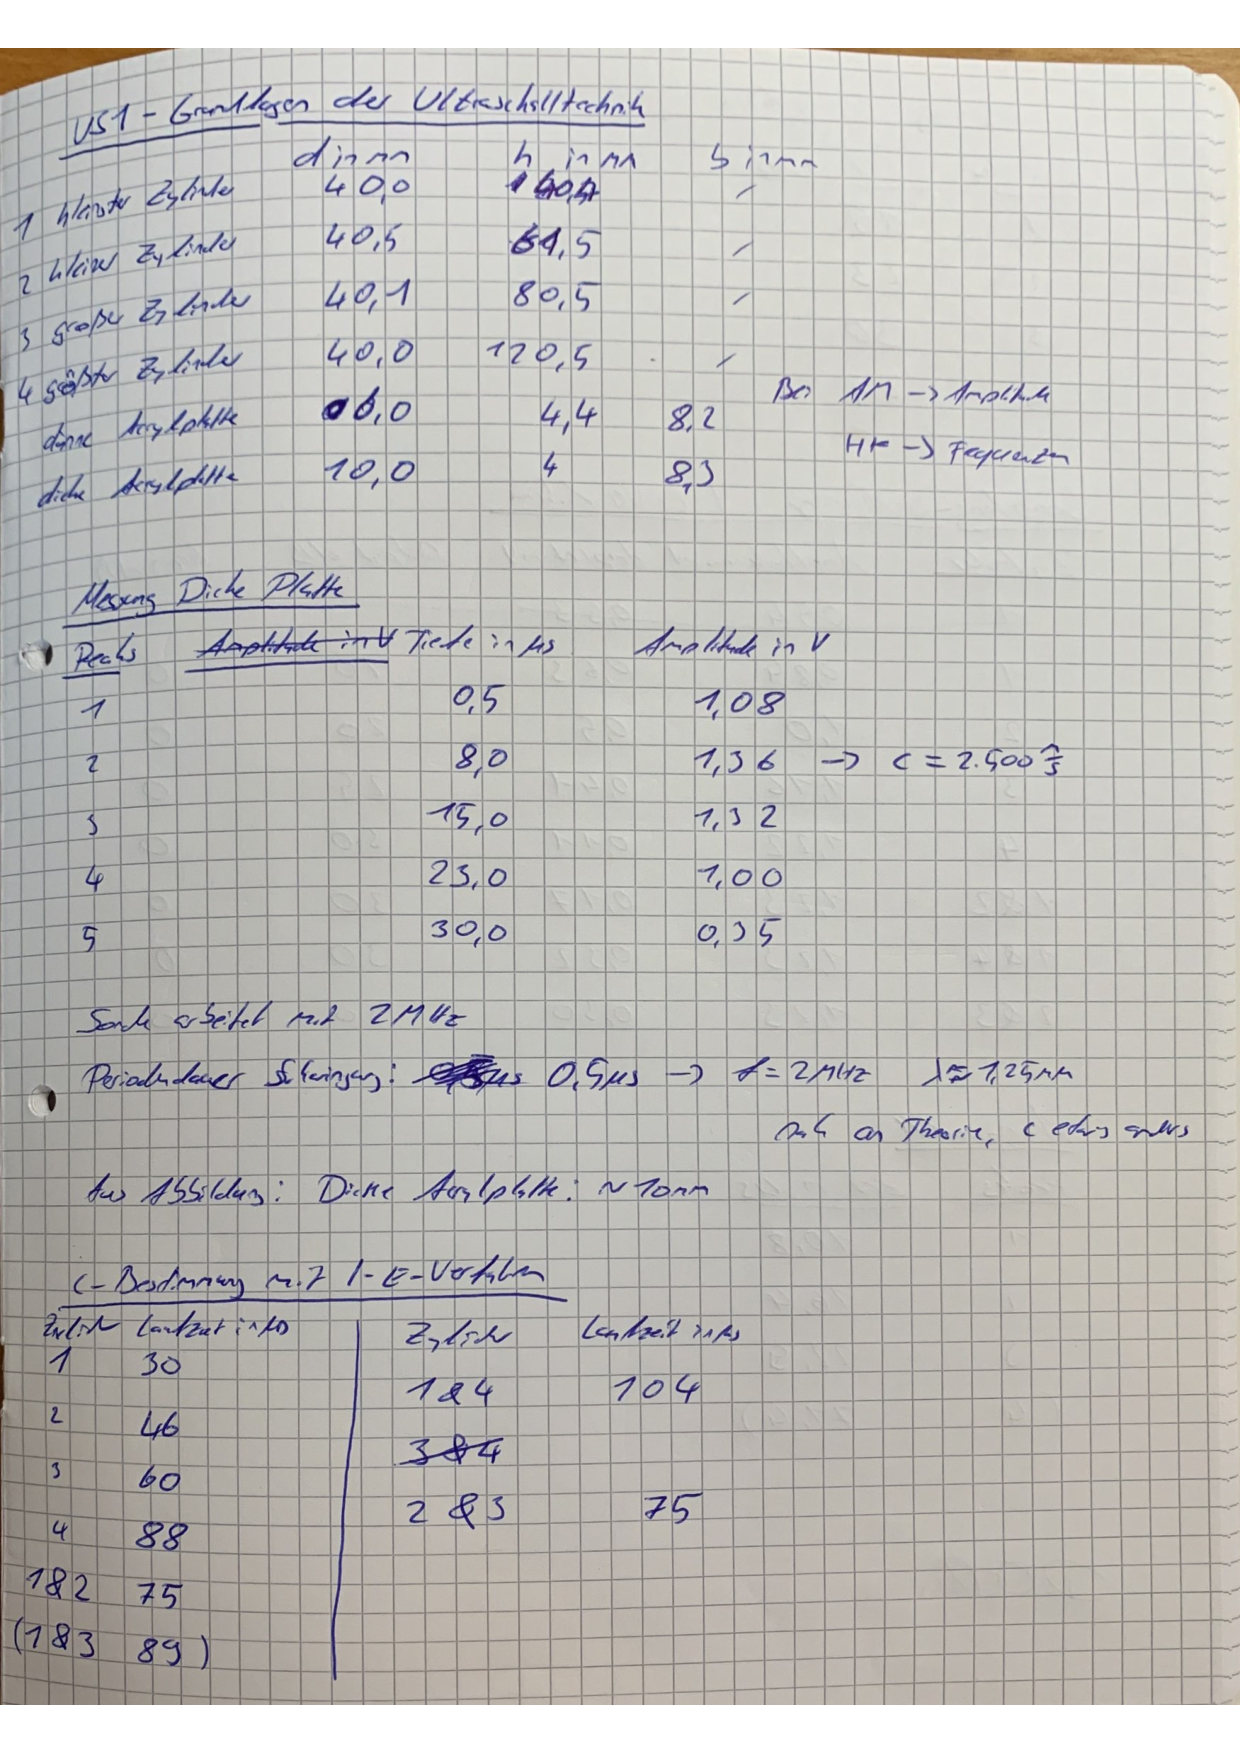
\includegraphics[height=18cm]{content/Originaldaten/Originaldaten_1.pdf}
\newpage
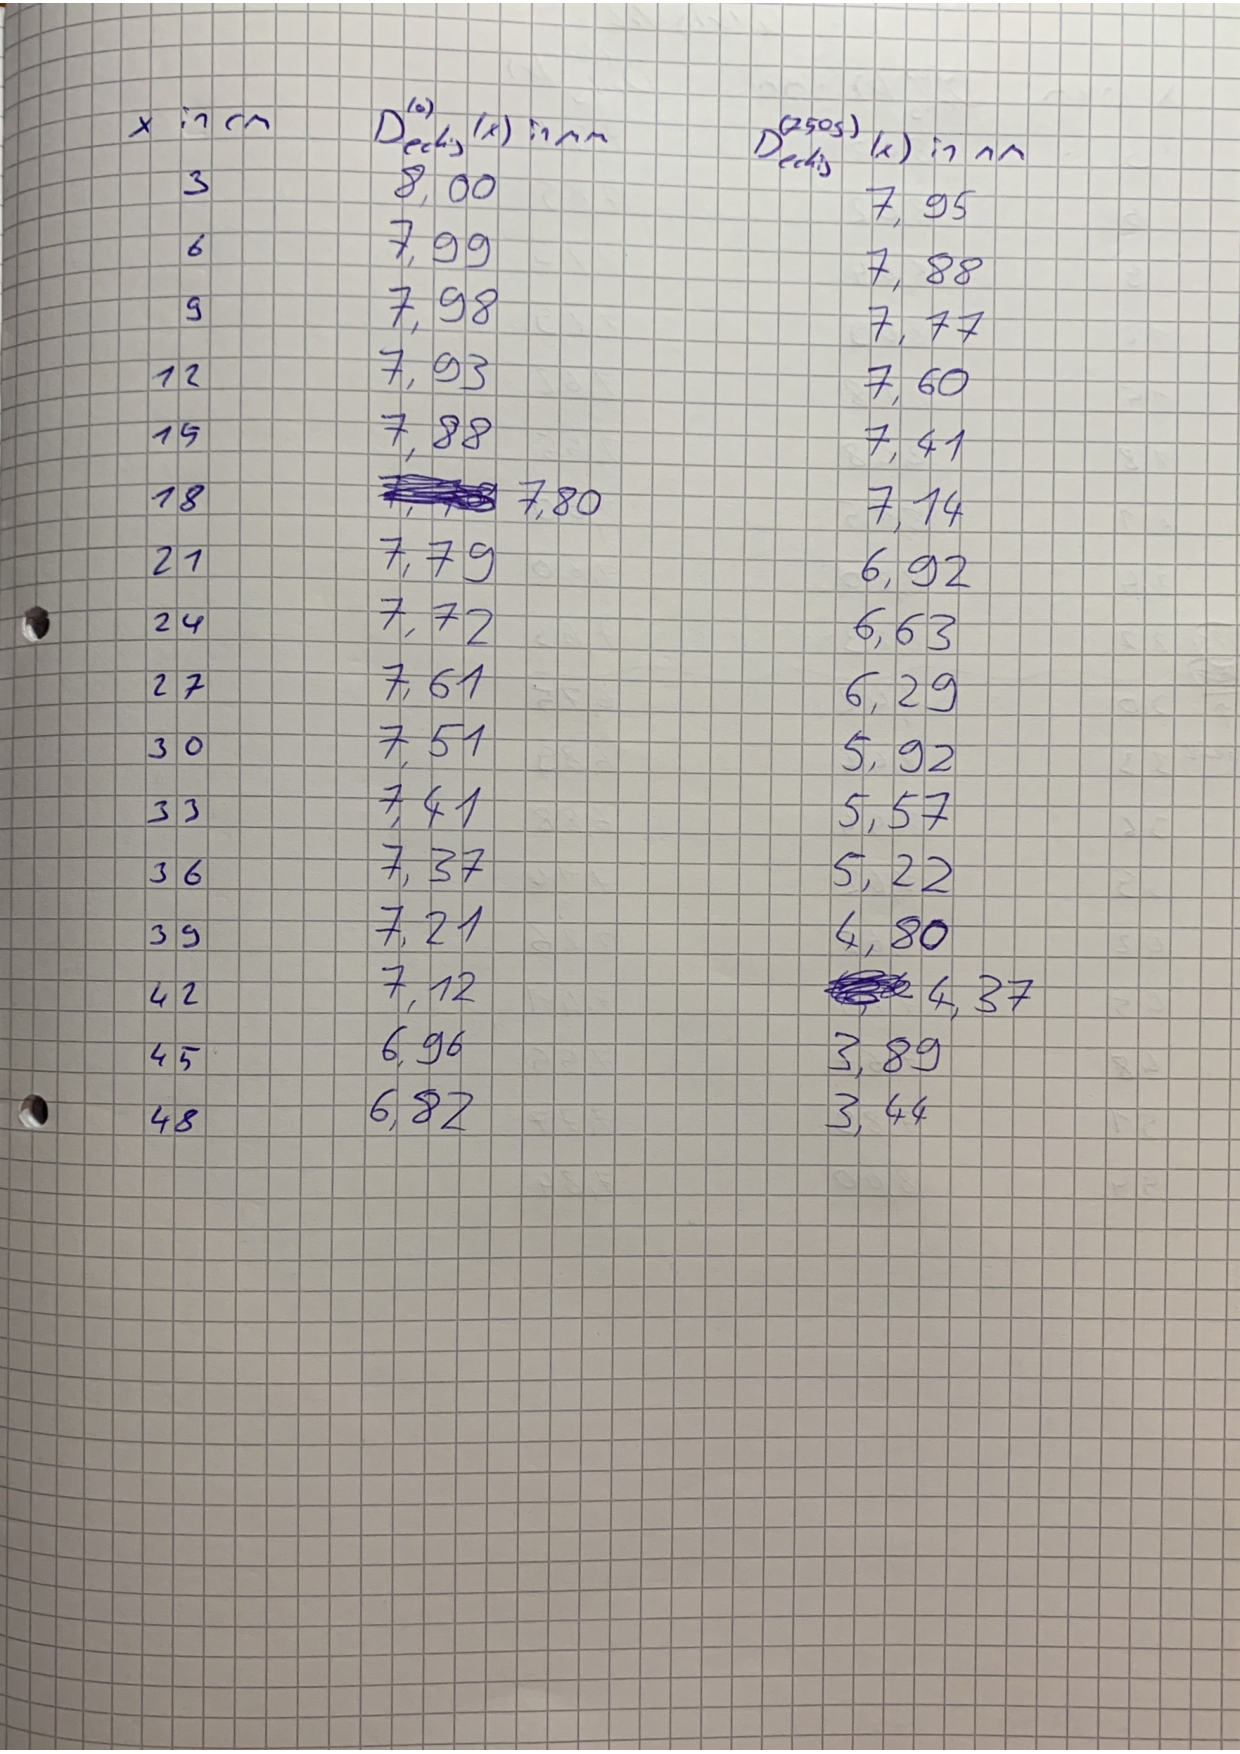
\includegraphics[height=18cm]{content/Originaldaten/Originaldaten_2.pdf}
\end{document}
